\documentclass[11pt]{article}
\usepackage[margin=1in]{geometry}
\usepackage{amsmath,amssymb}
\usepackage{parskip}
\usepackage{graphicx}
\usepackage{booktabs}


\begin{document}

\begin{center}
{\Large\bfseries Homework 3}\\[0.35em]
{\small Xingming Li \quad ID: 1432037}\\[0.2em]
{\small ECON*6020 Macroeconomic Theory I}
\end{center}

\hrule
\medskip

\textbf{Model.}
\begin{gather*}
\max \int_0^\infty \frac{\hat c_t^{\,1-\theta}}{1-\theta}\, e^{-[\rho-n-(1-\theta)x]t}\,dt
\qquad \text{s.t.} \qquad
\dot{\hat k}_t = \hat k_t^{\alpha} - (\delta+n+x)\hat k_t - \hat c_t .
\end{gather*}
Everything is in effective labour units: $\hat k_t = K_t/(A_tL_t)$, $\hat y_t = \hat k_t^{\alpha}$, and
$A_t = A_0e^{xt}$. From the Hamiltonian in class, the equilibrium is given by the Euler equation and the
law of motion for capital:
\begin{align*}
\frac{\dot{\hat c}_t}{\hat c_t} &= \frac{1}{\theta}\big[\alpha \hat k_t^{\alpha-1} - \delta - \rho - \theta x\big], \\
\dot{\hat k}_t &= \hat k_t^{\alpha} - (\delta+n+x)\hat k_t - \hat c_t .
\end{align*}
Setting both to zero gives the steady state
\[
\hat k_{ss} = \Big(\frac{\alpha}{\delta+\rho+\theta x}\Big)^{\frac{1}{1-\alpha}}, \qquad
\hat c_{ss} = \hat k_{ss}^{\alpha} - (\delta+n+x)\hat k_{ss}, \qquad
s_{ss} = \frac{(\delta+n+x)\hat k_{ss}}{\hat k_{ss}^{\alpha}} = \frac{\alpha(\delta+n+x)}{\delta+\rho+\theta x}.
\]

% ------------------------------------------------------------------
\section*{(1) Calibration of $\theta$ and the long-run interest rate}

The parameters are $\rho=0.01$, $n=0.01$, $x=0.02$ (income per capita grows at $x$ in the long run),
$\delta=0.05$, $\alpha = 1-\tfrac23 = \tfrac13$ and $A(0)=1$. That leaves $\theta$ as the only unknown.
I pick it so that the steady-state investment--GDP ratio in the model equals the $25\%$ in the data:
\begin{align*}
0.25 = \frac{\alpha(\delta+n+x)}{\delta+\rho+\theta x}
&\;\Longrightarrow\;
\delta+\rho+\theta x = \frac{\alpha(\delta+n+x)}{0.25} = \frac{\tfrac13(0.08)}{0.25} = 0.10\overline{6} \\
&\;\Longrightarrow\;
\theta = \frac{0.10\overline{6} - 0.05 - 0.01}{0.02} = \frac{7}{3} \approx 2.33 .
\end{align*}
We also need $\rho-n-(1-\theta)x>0$ for utility to be bounded. Here it is
$0.01-0.01+\tfrac43(0.02) = 0.0267>0$, so this is fine.

\textbf{Long-run interest rate.} In the steady state $\dot{\hat c}=0$, so the Euler equation gives
\[
r_{ss} = \alpha\hat k_{ss}^{\alpha-1} = \delta+\rho+\theta x = 0.10\overline{6},
\qquad
r_{ss}-\delta = \rho + \theta x = 0.01 + \tfrac73(0.02) \approx 0.0567 .
\]
The rental rate is about $10.7\%$ and the net real interest rate is about $5.7\%$ per year. For later
use, $\hat k_{ss} = (3.125)^{3/2}\approx 5.52$, $\hat y_{ss}\approx 1.77$ and $\hat c_{ss}\approx 1.33$.

% ------------------------------------------------------------------
\section*{(2) Transitional dynamics from $\hat k_0 = \tfrac14\hat k_{ss}$}

The system is nonlinear, so I solve for the saddle path numerically in \texttt{HW3.m}. The method is
reverse shooting. I start very close to $(\hat k_{ss},\hat c_{ss})$ along the stable eigenvector and run
the two equations backward in time (RK4). Going backward, the saddle path is stable, so this traces out
$\hat c(\hat k)$. Then I simulate forward from $\hat k_0 = \hat k_{ss}/4 \approx 1.38$ and compute
\[
s_t = 1 - \frac{\hat c_t}{\hat y_t}, \qquad
y_t = \frac{Y_t}{L_t} = A_t\hat k_t^{\alpha} = e^{xt}\hat k_t^{\alpha} .
\]

\begin{figure}[h]
\centering
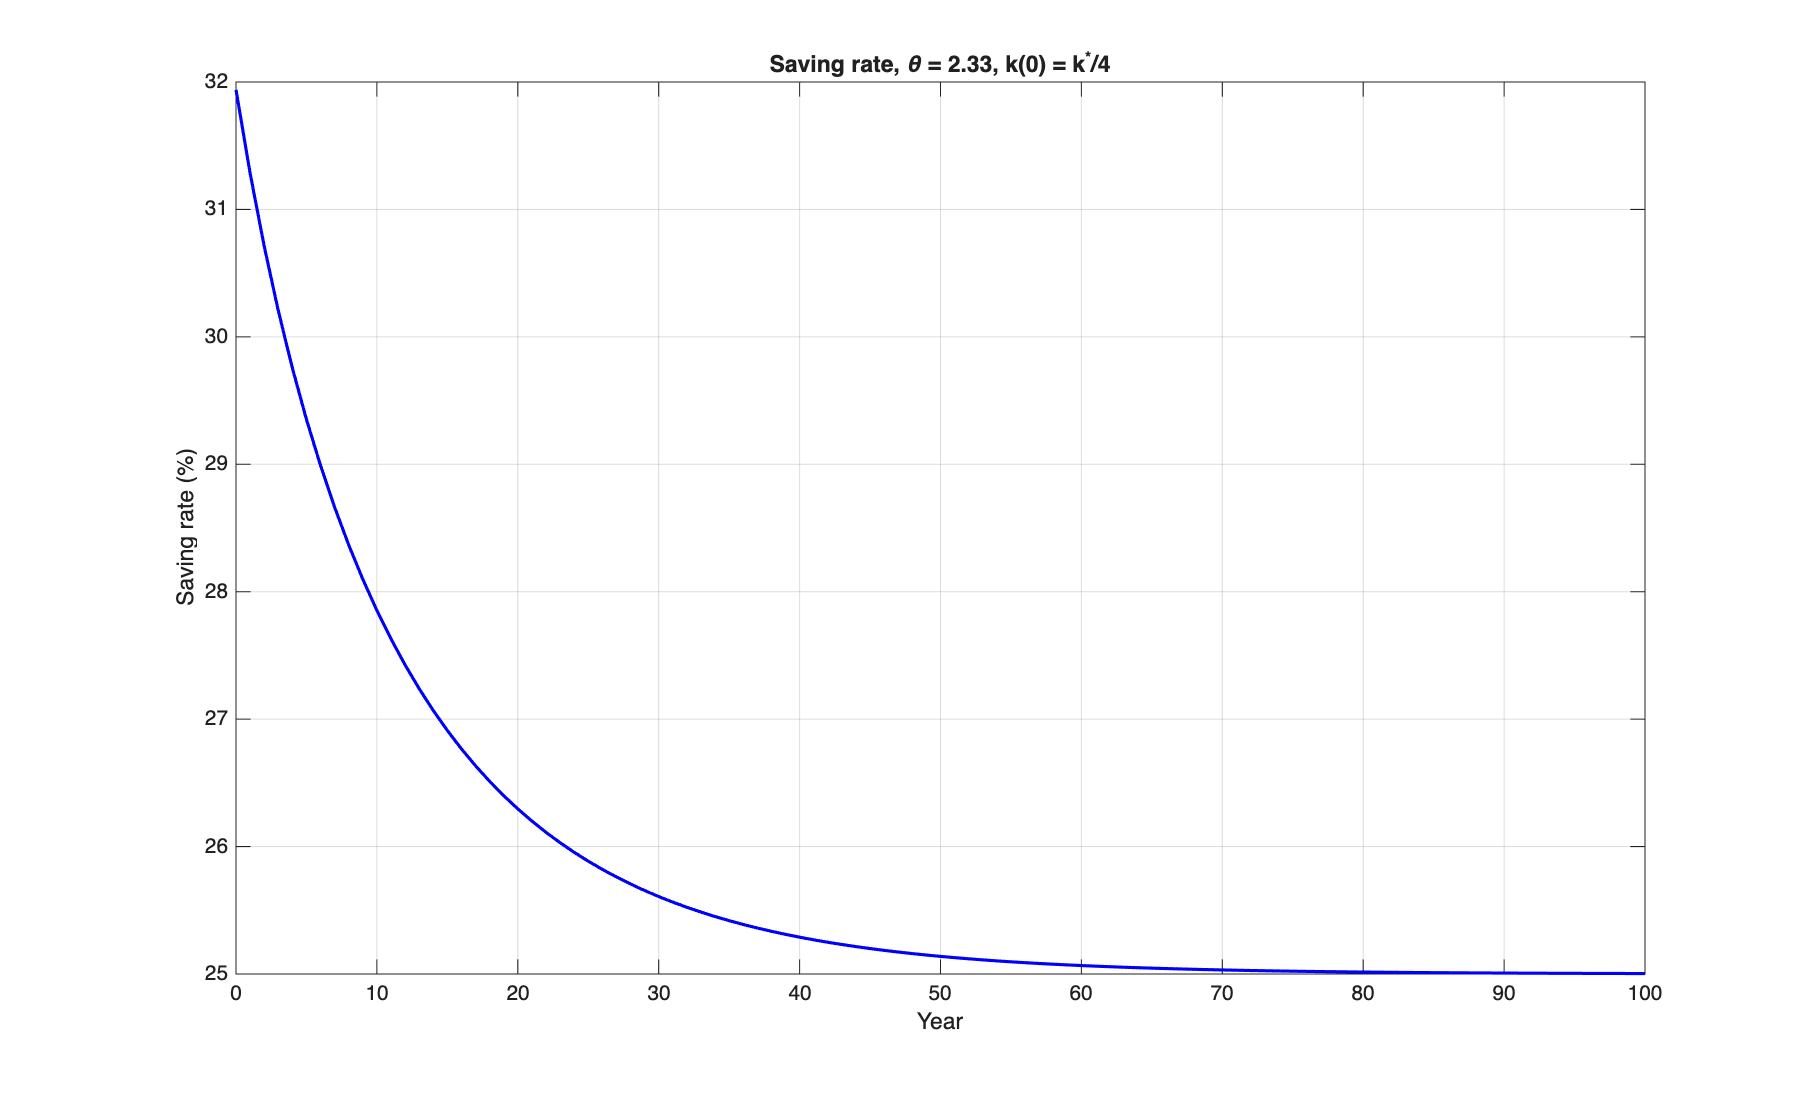
\includegraphics[width=0.49\textwidth]{hw3_saving.png}
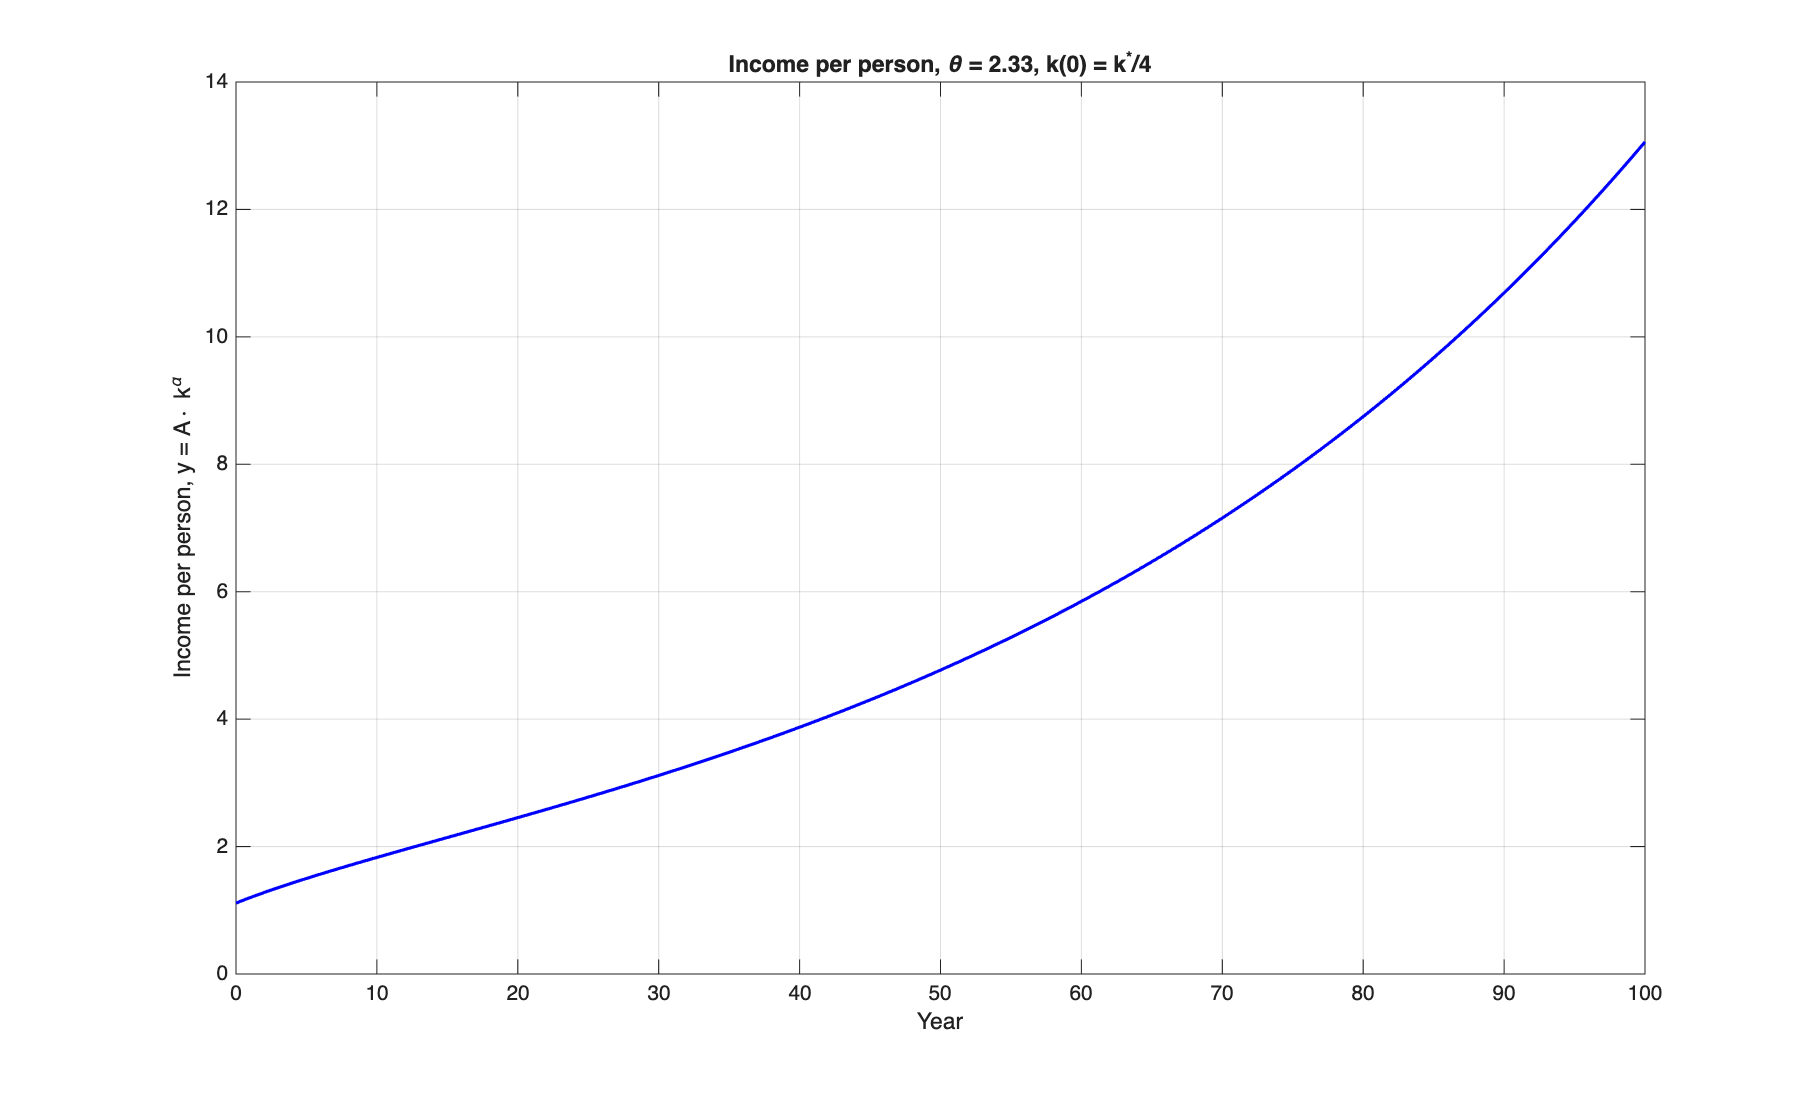
\includegraphics[width=0.49\textwidth]{hw3_income.png}
\end{figure}

\begin{figure}[h]
\centering
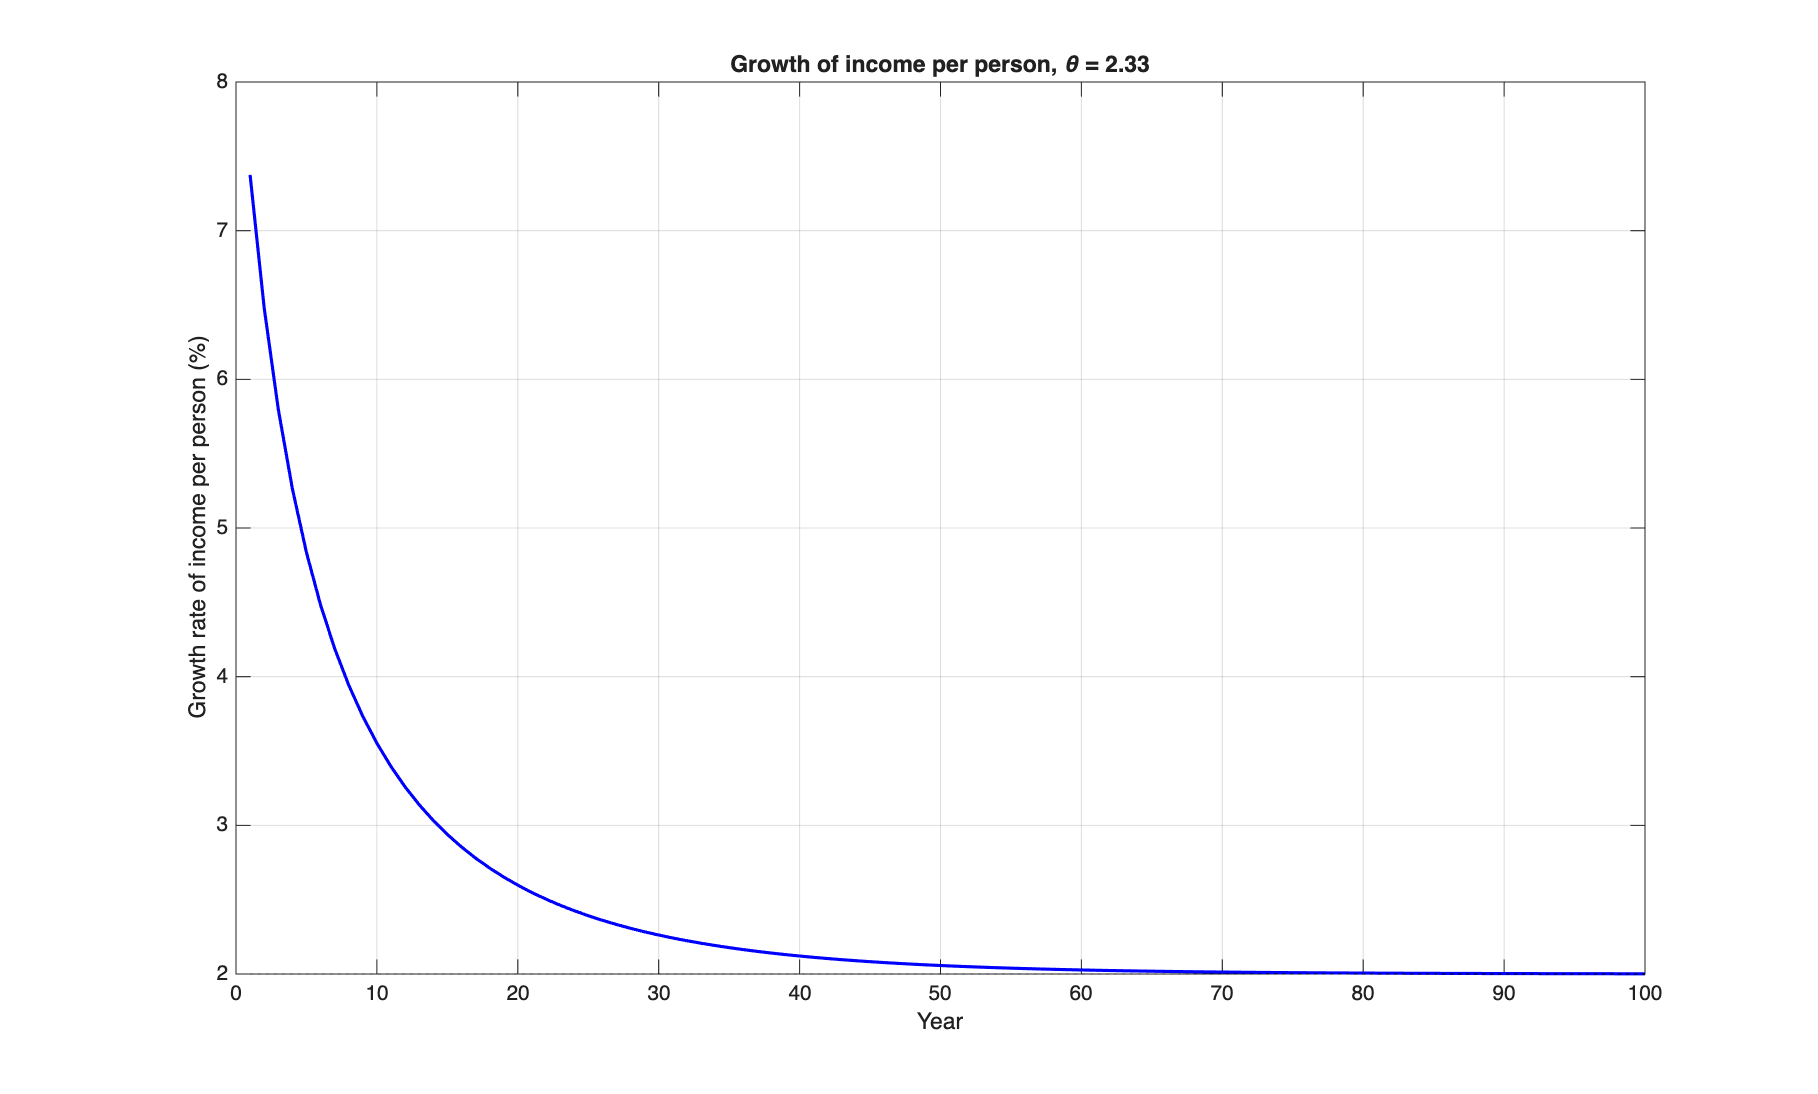
\includegraphics[width=0.6\textwidth]{hw3_growth.png}
\end{figure}

\begin{center}
\begin{tabular}{lcccccccc}
\toprule
Year & 0 & 1 & 5 & 10 & 20 & 30 & 50 & 100 \\
\midrule
Saving rate (\%) & 31.9 & 31.3 & 29.4 & 27.9 & 26.3 & 25.6 & 25.1 & 25.0 \\
Growth of $y_t$ (\%) & -- & 7.4 & 4.8 & 3.6 & 2.6 & 2.3 & 2.1 & 2.0 \\
\bottomrule
\end{tabular}
\end{center}

\textbf{Growth rate of income per person.} Income per person goes from about $1.11$ to $13.1$ over the
100 years. Since $y_t = e^{xt}\hat k_t^{\alpha}$, its growth rate is
$\gamma_y = x + \alpha\,\dot{\hat k}/\hat k$. At the start capital is scarce and its return is high, so
$\hat k$ grows fast and income grows about $7.4\%$ in the first year. As capital builds up,
diminishing returns slow down $\dot{\hat k}/\hat k$. Growth keeps falling until it settles at the
technology growth rate $x=2\%$. This is the usual conditional convergence result.

\textbf{Saving rate.} The saving rate starts at about $32\%$ and falls slowly to $25\%$. When
$\hat k$ is low, $r=\alpha\hat k^{\alpha-1}$ is very high, so saving pays off a lot. There are two forces
here. The substitution effect says save more while the return is high. The income effect says
households know they will be much richer later, so they want to consume more now. With $\theta = 7/3$,
the elasticity $1/\theta\approx0.43$ is fairly large, so the substitution effect wins. As $\hat k$ rises
and $r$ falls, saving becomes less attractive and the saving rate drops.

% ------------------------------------------------------------------
\section*{(3) Speed of convergence}

Linearize the system around $(\hat k_{ss},\hat c_{ss})$, using
$\alpha\hat k_{ss}^{\alpha-1}=\delta+\rho+\theta x$:
\[
\begin{bmatrix}\dot{\hat k}_t\\ \dot{\hat c}_t\end{bmatrix}
\approx
\underbrace{\begin{bmatrix}
\zeta & -1\\[2pt]
-\dfrac{\hat c_{ss}}{\theta}\,\alpha(1-\alpha)\hat k_{ss}^{\alpha-2} & 0
\end{bmatrix}}_{J}
\begin{bmatrix}\hat k_t-\hat k_{ss}\\ \hat c_t-\hat c_{ss}\end{bmatrix},
\qquad
\zeta \equiv \alpha\hat k_{ss}^{\alpha-1}-(\delta+n+x) = \rho-n-(1-\theta)x .
\]
Since $\det J<0$, one eigenvalue is positive and one is negative, which is the saddle path. The speed
of convergence $\beta$ is minus the negative eigenvalue:
\[
\beta = \frac12\Big[\sqrt{\zeta^2 + 4\,\tfrac{\hat c_{ss}}{\theta}\,\alpha(1-\alpha)\hat k_{ss}^{\alpha-2}}
          \;-\; \zeta\Big].
\]
Plugging in $\hat c_{ss}$ and $\hat k_{ss}$ gives the closed form
\[
2\beta = \bigg\{\zeta^2 + 4\,\frac{1-\alpha}{\theta}(\rho+\delta+\theta x)
         \Big[\frac{\rho+\delta+\theta x}{\alpha} - (n+x+\delta)\Big]\bigg\}^{1/2} - \zeta .
\]
With $\zeta = 0.0267$, $\hat c_{ss}=1.326$, $\hat k_{ss}=5.524$ and $\theta=7/3$:
\[
\beta = \tfrac12\big[\sqrt{0.0267^2 + 4(0.00731)} - 0.0267\big] \approx 0.073 .
\]
Near the steady state, about $7.3\%$ of the gap $\ln\hat k_t - \ln\hat k_{ss}$ closes each year, so
the half-life is $\ln 2/\beta \approx 9.5$ years.

\textbf{Comparison with Solow.} With the same parameters and $s=0.25$, the Solow model gives
\[
\beta_{Solow} = (1-\alpha)(\delta+n+x) = \tfrac23(0.08) \approx 0.053 .
\]
So the Ramsey economy converges faster, $7.3\%$ versus $5.3\%$, even though both have the same
steady state. The difference comes from saving. In Solow the saving rate is stuck at $25\%$. In Ramsey,
part (2) shows that saving is above $25\%$ when the economy is below its steady state. A poor Ramsey
economy invests more than a poor Solow economy, so it catches up faster. This depends on
$\theta < 1/s_{ss} = 4$, which I show in part (4). If $\theta$ were equal to $1/s_{ss}$, saving would
be constant and the two speeds would be the same. If $\theta$ were above $1/s_{ss}$, Ramsey would
actually be slower than Solow.

% ------------------------------------------------------------------
\section*{(4) Saving rate with $\theta=9$ and $\theta=20$}

A larger $\theta$ raises $\delta+\rho+\theta x$ and lowers the steady state. So each run starts from
its own $\hat k_0 = \hat k_{ss}(\theta)/4$:

\begin{center}
\begin{tabular}{lcccccc}
\toprule
$\theta$ & $r_{ss}$ & $\hat k_{ss}$ & $s_{ss}$ & $1/\theta$ & $s_0$ & $\beta$ \\
\midrule
$7/3$ & 0.107 & 5.52 & 0.250 & 0.429 & 0.319 & 0.073 \\
$9$   & 0.240 & 1.64 & 0.111 & 0.111 & 0.111 & 0.053 \\
$20$  & 0.460 & 0.62 & 0.058 & 0.050 & 0.053 & 0.047 \\
\bottomrule
\end{tabular}
\end{center}

\begin{figure}[h]
\centering
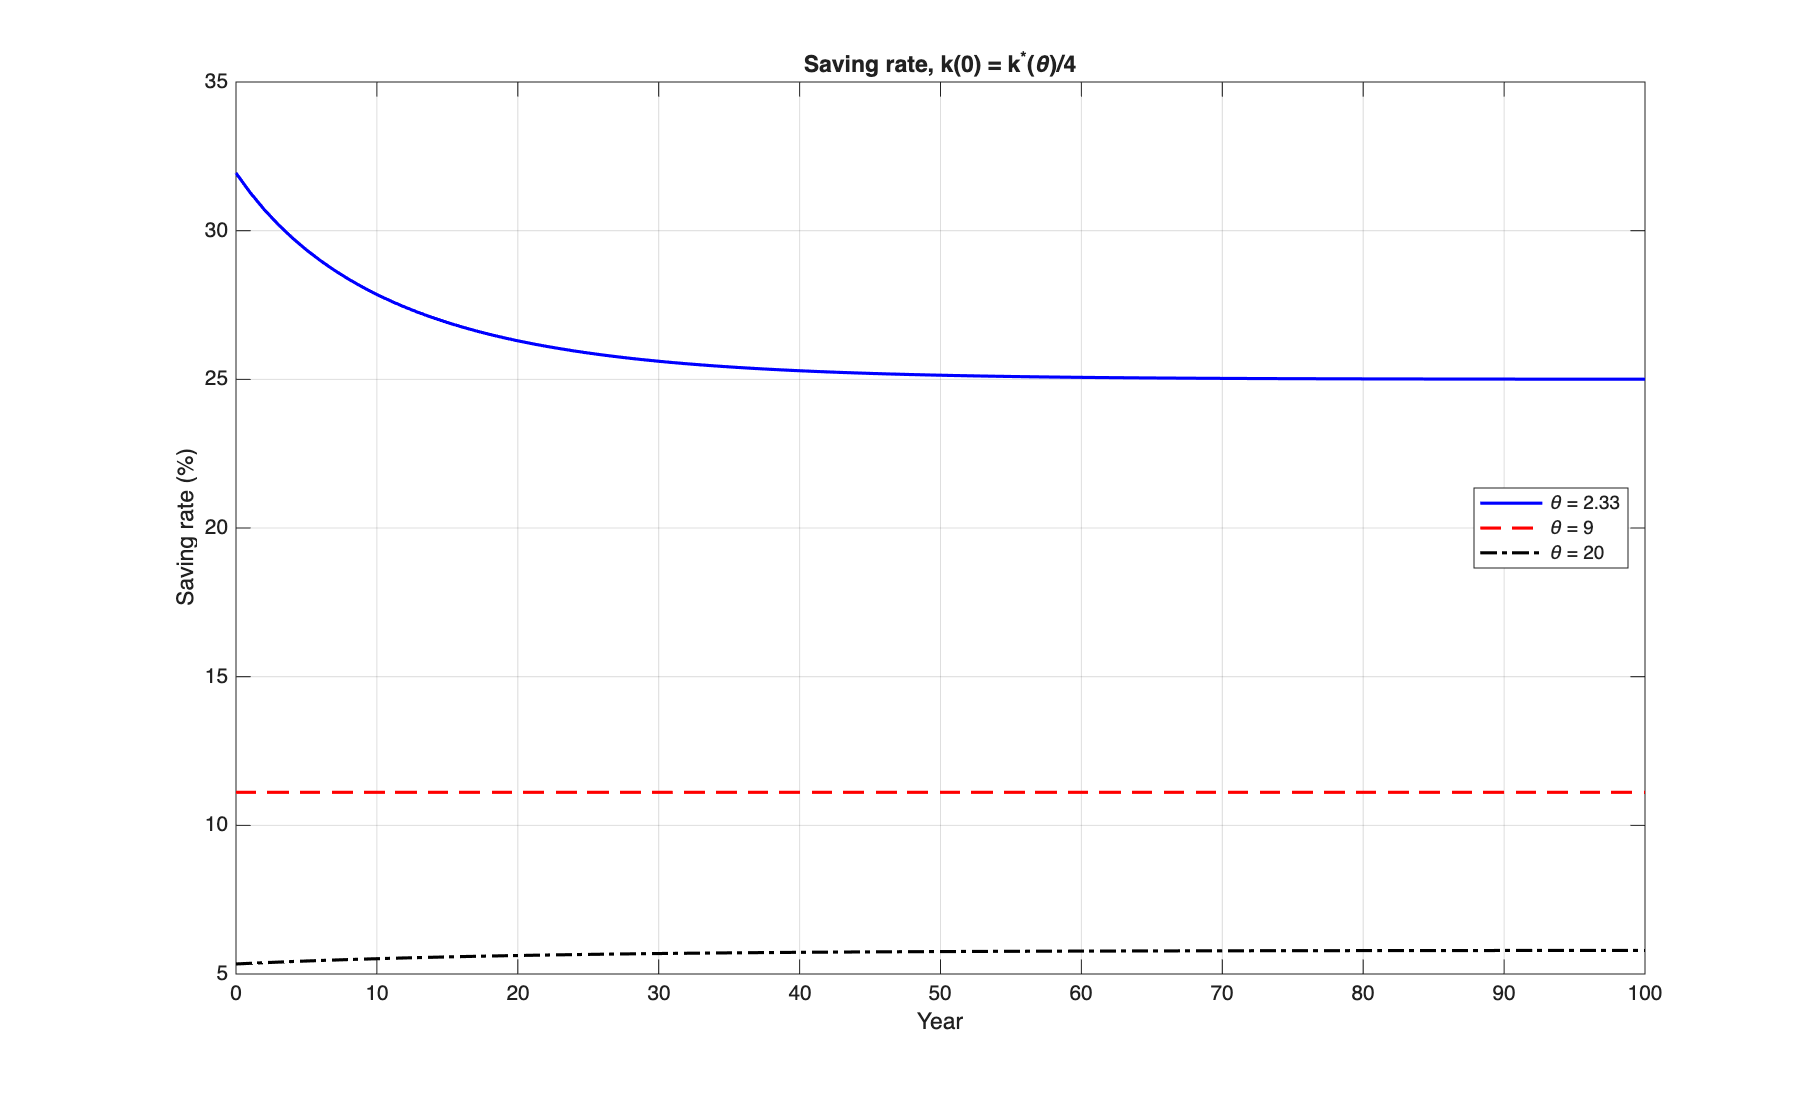
\includegraphics[width=0.7\textwidth]{hw3_saving_theta.png}
\end{figure}

\textbf{When is the saving rate constant?} Suppose $s_t=s$ for all $t$. Then
$\hat c_t=(1-s)\hat k_t^{\alpha}$, so
$\dot{\hat c}/\hat c = \alpha\,\dot{\hat k}/\hat k = \alpha s\hat k^{\alpha-1} - \alpha(\delta+n+x)$.
The Euler equation says
$\dot{\hat c}/\hat c = \tfrac1\theta\alpha\hat k^{\alpha-1} - \tfrac1\theta(\delta+\rho+\theta x)$.
For these to agree at every $\hat k$, the coefficients on $\hat k^{\alpha-1}$ and the constants must
both match:
\[
s = \frac1\theta \qquad\text{and}\qquad \frac1\theta = \frac{\alpha(\delta+n+x)}{\delta+\rho+\theta x} = s_{ss}.
\]
So the saving rate stays constant along the transition exactly when $\theta = 1/s_{ss}$.

\textbf{(i) $\theta=9$.} Here $s_{ss} = \frac{\frac13(0.08)}{0.05+0.01+0.18} = \frac19$, which is exactly
$1/\theta$. This is the knife-edge case, and the saving rate stays flat at $11.1\%$ the whole way. The
substitution and income effects cancel out, so the economy behaves just like a Solow model with
$s=1/9$. Its convergence speed is also the Solow value, $(1-\alpha)(\delta+n+x)=0.053$.

\textbf{(ii) $\theta=20$.} Now $1/\theta = 0.05 < s_{ss} = 0.058$, and the picture flips. Saving starts
low, at about $5.3\%$, and rises slowly to $5.8\%$. With $1/\theta = 0.05$, households barely respond to
the interest rate and mostly care about smoothing consumption. A poor economy expects much higher income
later, so people keep consumption high today and save little. Here the income effect beats the
substitution effect. As the economy gets richer, that motive fades and the saving rate goes up. Because
saving is low exactly when capital is scarce, convergence is slower than in Solow ($\beta\approx0.047$).

\end{document}
